\documentclass[a4paper]{article}

\usepackage{INTERSPEECH2018}
\usepackage{tikz}
\usepackage{url}
\usepackage{blindtext}
\usetikzlibrary{shapes,arrows,positioning}

\tikzstyle{block} = [draw, fill=white, rectangle, 
    minimum height=3em, minimum width=6em]
\tikzstyle{sum} = [draw, fill=white, circle, node distance=1cm]
\tikzstyle{input} = [coordinate]
\tikzstyle{output} = [coordinate]
\tikzstyle{pinstyle} = [pin edge={to-,thin,black}]

\title{Multi-speaker articulatory-to-acoustic speech synthesis with
deep neural networks}
\name{Bence Halpern$^1$$^2$, Rob J. J. H. van Son$^1$, Michiel W. M.
  van den Brekel$^1$$^2$}
%The maximum number of authors in the author list is twenty. If the number of contributing authors is more than twenty, they should be listed in a footnote or in acknowledgement section, as appropriate.
\address{
  $^1$NKI-AVL, Amsterdam\\
  $^2$ACLC,University of Amsterdam, The Netherlands}
\email{b.halpern@nki.nl, r.v.son@nki.nl}

\begin{document}

\maketitle
% 
\begin{abstract}
  \blindtext[1]
\end{abstract}
\noindent\textbf{Index Terms}: computational paralinguistics, articulatory-to-acoustic
speech synthesis, deep learning, pathological speech

\section{Introduction}

Understading how articulation affects speech is a central question in speech
research. The source-filter model was one of the first models to tackle this
problem by noting that speech production could be described by
the geometry of the vocal tract and the glottal wave. Mathematically,
the source-filter model synthetises speech by exciting an autoregressive (AR) model with a
signal, where the AR coefficients capture the geometry of the
vocal tract, which is also represented by an area function \cite{Benesty2009}. 

\begin{figure}[t]
  \begin{center}
    \scalebox{0.75}{
  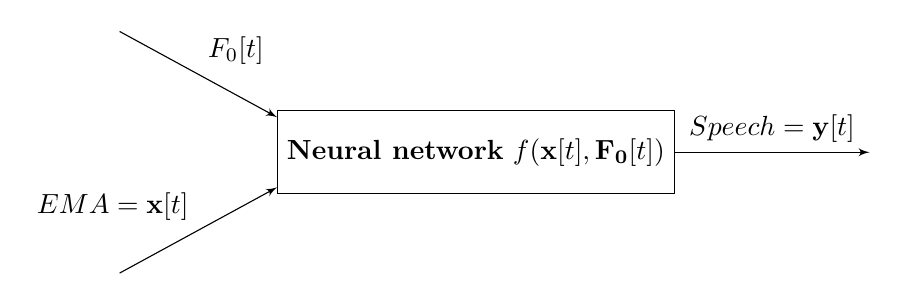
\begin{tikzpicture}[auto, node distance=5cm,>=latex']
    \node [input] (f0) {$F_0$};
  \node [block, below right = 1 cm and 2 cm of f0] (predictor) { \textbf{Neural network} $f(\mathbf{x}[t], \mathbf{F_0}[t]) $ };
  \node [input, name=input, right of = predictor] (speech) {Speech};
    \node [input, below left = 1 cm and 2 cm of predictor] (ema) {};
    \draw [->] (f0) -- node {$ F_0[t] $}   (predictor.170);
    \draw [->] (ema) -- node {$ \text{EMA} = \mathbf{x}[t] $}   (predictor.190);
    \draw [->] (predictor) -- node {$ \text{Speech} = \mathbf{y}[t] $} (speech);
  \end{tikzpicture}
}

    \scalebox{0.75}{
  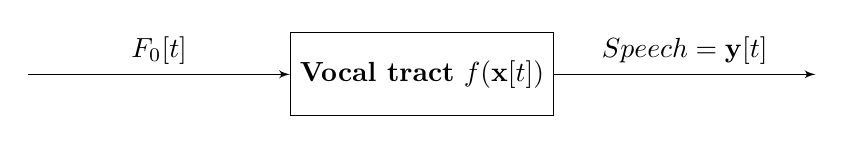
\begin{tikzpicture}[auto, node distance=5cm,>=latex']
    \node [input] (f0) {$F_0$};
  \node [block, right of = f0] (predictor) { \textbf{Vocal tract} $f(\mathbf{x}[t]) $ };
  \node [input, name=input, right of = predictor] (speech) {Speech};
    \draw [->] (f0) -- node {$ F_0[t] $}   (predictor);
    \draw [->] (predictor) -- node {$ \text{Speech} = \mathbf{y}[t] $} (speech);
  \end{tikzpicture}
 }
 \caption{Black box diagram showing the parallelities of a neural network
   based model with a source-filter model}
  \label{fig1}
    \end{center}
  \end{figure}

Recently, deep learning methods became popular
to understand articulation. These methods use a measurement tool,
called electromagnetic articulography to obtain articulation data 
\cite{Aryal2016} \cite{Taguchi} \cite{Liu2018} along with recurrent
neural networks, which are neural networks that are able to deal with
the sequential nature of data. Data-driven methods became of interest also
in real-time speech synthesis. The efficacy of real-time speech synthesis
has been investigated using a tool called permanent magnetic articulography
by Gonzalez et al \cite{Gonzalez2017}, which gave understandable
speech.

The conclusion of these endeavours were that while it is possible to
predict some of the pitch from articulation, the quality suffers.
It is, however, possible to obtain satisfactory values for the
cepstral quality.



In the author's broader research, the aim is to demonstrate how pathologies in
articulation are translated to speech. In some types of pathological
speech the laryngeal function remains intact, meaning the \( F_0 \)
remains unchanged. This means, by knowing the original pitch and the
pathological deviations in articulation, it should be possible to
synthetise pathological speech.

The idea with MFCCs is to separate vocal tract information from the excitation
information. Thus based on the electrode signals of the vocal tract configuration
it should be possible to predict part of the spectra only dependent on the vocal
tract configuration.

The main contributions of this paper are,
\begin{itemize}
\item a set of benchmarks for multi-speaker articulatory to acoustic synthesis
\item estimation on how much data would be needed to construct a better model
\item an example of how to construct pathological speech using this framework
\end{itemize}

Our code is also available as a Github repository on the link
\url{https://github.com/karkirowle/vocoder-clean}.

\section{Method}
\subsection{Electromagnetic articulography}

Electromagnetic articulography (EMA) is a measurement technology which uses
sensor coils which are placed on the different articulators in the vocal tract.
Using this technology it is possible to record the displacement of the articulators
which can then be used to predict speech which is simultaneously recorded.

The electrodes are placed on the MNGU0 \cite{Richmond2011} and MOCHA-TIMIT dataset on a total
of seven positions. The two datasets have not recorded entire the
same channels, so Table \ref{tab:electrodes} include the alignment
that has been used.
\begin{table}[th]
  \label{tab:electrodes}
  \caption{Articulatory information recorded in datasets}
  \centering
  \begin{tabular}{ r r }
    \toprule
    \textbf{MNGU0} & \textbf{MOCHA-TIMIT} \\
    \midrule
    Tongue dorsum (T3) & Tongue dorsum (T3) \\
    Tongue blades (T2) & Tongue blades (T2) \\
    Tongue tip (T1) & Tongue tip (T1) \\
    Lower incisor (T3) & Jaw \\
    Upper incisor & Nose \\
    Upper lip & Upper lip \\
    Lower lip & Lower lip \\
    \bottomrule
    \end{tabular}
\end{table}

TODO: Decide whether you want to leave out the lower incisor or jaw

\begin{figure}[t]
  \begin{center}
    \scalebox{0.50}{\input{init_pos.pgf}}
  \caption{The visualisation of electrode locations for all samples in
    the MNGU0 dataset at time point \( t = 0 \)}
\end{center}
\end{figure}
\subsection{Dataset}

The MNGU0 and the MOCHA-TIMIT dataset were used to obtain a total of
2274 samples, which were partitioned to training and validation set when
no hyperparameter optimisation was done. An additional test set was used
in case of hyperparameter optimisation. The dataset contains data from
three speakers, two British male and one British female. The recordings
from the microphones were 16kHz.

\subsection{Sampling}

It is important that the input and output sample rates of the different
datasets are matched, because otherwise, the input-output pairs contain
different amounts of information.  

The sampling frequency of the original EMA signals were 500 Hz, however
the MNGU0 was provided to us downsampled to 200 Hz. To match this frequency,
the sampling frequency of the MOCHA-TIMIT were also downsampled to 200 Hz.

For the MNGU0 dataset, NaN values occured when the measurement precision
was lose. These values were simply interpolated linearly.

To ease training, the input signals were either truncated or padded
so there were a total of \( T = 1000 \) samples for each training example.
For input signals which are shorter, it is assumed that the last part is
silence, so it is padded with the last element.

\subsection{Vocoder analysis}

Vocoder features were extracted with the PyWORLD vocoder \cite{Morise2016}
and compressed with the PySPTK toolkit available at \url{http://github.com/r9y9/pysptk}.
The period between consecutive frames were 5 miliseconds. The resulting 40 MFCC
and 1 power parameters were used to generatic static and delta parameters,
resulting in 82 parameters for the training. As the first step of the MFCC extraction \( \alpha
= 0.42 \) were used a pre-emphasis coefficient. The PyWORLD vocoder
also provides the $ F_0 $ and BAP values for synthesis, these were
explicitly given for the synthesis, due to the reasons stated in the
Introduction.

\subsection{Delay}
Previously \cite{Gonzalez2016}, the effect of delay on the
output signal were investigated. While it has been found that delay
is beneficial, the author's choice of function approximators are
restricted to acausal models, so it has been decided
not to use delay in our final implementation.

\subsection{Fundamental frequency interpolation}

Previously, it has been found beneficial to take the logarithm of the
pitch to obtain a continous \( F_0 \) curve.
When the logarithm is not defined, linear  interpolatation has been done. \cite{Gonzalez2017}
An alternative method also exists with exponential interpolation
which is described in \cite{Chen1997}. It has been decided that the
linear interpolation technique will be used. 

\subsection{Normalisation}

Exploratory data analysis indicated that the articulatory trajectories of
the datasets were on different scale and bias, so it was normalised
on a per speaker basis. The output MFCCs were normalised for each cepstral
coefficients.

\subsection{Neural network}

To approximate the functional relationship, the authors have decided to
train a Bidirectional Long-Short Term Memory based neural network \cite{Hochreiter1997}. 

For all BLSTM layers, the CuDNNLSTM implementation have been used to
improve efficiency, however this limits the activation function to be
stricly \( \text{tanh}(\cdot) \)

A LSTM is governed by the following equations,

\begin{equation}
  \mathbf{i}_{t} = \sigma ( \mathbf{W}_{xi} \mathbf{x}_{t} + \mathbf{W}_{hi}
  \mathbf{h}_{t-1} + \mathbf{W}_{ci} \mathbf{c}_{t-1} + \mathbf{b}_{i}),  
\end{equation}
\begin{equation}
  \mathbf{f}_{t} = \sigma ( \mathbf{W}_{xf} \mathbf{x}_{t} + \mathbf{W}_{hf}
  \mathbf{h}_{t-1} + \mathbf{W}_{cf} \mathbf{c}_{t-1} + \mathbf{b}_{f}), 
\end{equation}
\begin{equation}
  \mathbf{c}_{t} = \mathbf{f} \mathbf{c}_{t-1} + \mathbf{i}_{t} \text{tanh} ( \mathbf{W}_{hc}
  \mathbf{h}_{t-1} + \mathbf{b}_c),
\end{equation}
\begin{equation}
  \mathbf{o}_{t} = \sigma ( \mathbf{W}_{x0}\mathbf{x}_t + \mathbf{W}_{ho} \mathbf{h}_{t-1}
  + \mathbf{W}_{co}\mathbf{c}_{t} + \mathbf{b}_0 ),
\end{equation}
\begin{equation}
  \mathbf{h}_t = \mathbf{o}_{t} \text{tanh} ( \mathbf{c}_t ).
  \end{equation}

The exact architectures are described in the Section \ref{nnexperiment}.

\subsection{Synthesis}

Synthesis for the validation set is performed using the ground truth
parameters for the BAP and $ F_0 $ and only the spectral prediction is
benchmarked.

\begin{table}[th]
  \caption{Comparison of preprocessing techniques}
  \label{tab:example}
  \centering
  \footnotesize
  \begin{tabular}{ r r r r }
    \toprule
    \textbf{Author} & \textbf{Liu} & \textbf{Taguchi} & \textbf{Gonzalez} \\
    \midrule
    \textbf{EMA/PMA} & EMA & EMA & PMA \\
    \textbf{MFCC} & 40 + 1 & 40 + 1 & 24 + 1 \\
    \textbf{Delta} & No & Yes & Yes \\
    \textbf{EMA sampling} & 200 Hz & 200 Hz & 100 Hz* \\
    \textbf{Input standardisation} & Yes & N/A  & Yes \\
    \textbf{Trajectory smoothing} & No & Yes  & No \\
    \textbf{Output standardisation} & Yes & Yes & Yes \\
    \textbf{Vocoder} & STRAIGHT & WORLD  & STRAIGHT \\
    \bottomrule
    
  \end{tabular}
  *Upsampled to 200 to match analysis rate
\end{table}

\section{Experiment}

\subsection{Neural network experiments} \label{nnexperiment}

Three recurrent neural networks architectures were trained based on previous
papers tackling similiar problems.

Based on \cite{Liu2018}, a bidirectional LSTM was trained with four layers.
The final layer was a fully connected layer matching the output dimensions.
This neural network was trained using stochastic gradient descent and
a learning rate of \( \alpha = 0.01 \).

Another publication \cite{Taguchi} used a neural networks with three fully
connected layers with 128 hidden units, each layer has a linear activation
function, which is followed by Layer Normalisation and a sigmoid activation
function. This is followed by two BLSTM layers with 256 hidden units. Finally,
a fully connected layer is used. This neural network was trained using Grave's RMSProp (TODO: ref),
with a learning rate of \( \alpha = 0.01 \) .

Finally, another BLSTM was trained based on the architecture of
\cite{Liu2018}, but using Adam as an optimiser \cite{Kingma2015}.

Determining a good set of architecture and parameter settings is the most difficult part of
the experiment design. Bidirectional LSTMs have performed the best on predicting the MFCC spectra in
all related papers. Taguchi uses fully-connected layers and while it not justified in the paper, it
is reasonable to assume that this does pre-processing of the time-series. 

It can be easily seen mathematically that after after the last LSTM layer, a fully connected layer is also needed as this acts as a linear regression based on the LSTM parameters. This is because the range of the activation function is not sufficient to capture the range of the normalised MFCCs. It is possible to introduce some structural bias by using the same linear regression from each frame, somewhat limiting complexity. 

In terms of the optimisation, Adam and Graves's RMSProp is preferred, which is not surpsing due to the
fact that these known to be better for optimising non-stationary objectives. With the SGD,
learning rate scheduling had to be used. 

In order to choose the best architecture, all of them have been reimplemented with slight modifications.
This is a better practice, because the MCD's were interpreted differently on the different papers, i.e the error in the silence frames were not taken into consideration. All of them were compared on the mngu0 dataset. The best performing architecture have been retrained on the full dataset, using the preprocessing techniques mentioned above, and an MCD of 5.48 have been obtained.


A possible approach is to use transfer learning to get better performance.

The idea is either to freeze the initial model trained on the mngu0, then use pre-processing
layers to learn the feature mappings. 
Some valid questions: generalisation by validating on certaind datasets.

\begin{table}[th]
  \caption{Transfer learning comparison with single speaker models}
  \label{tab:transfer}
  \centering
  \footnotesize

  \begin{tabular}{ r r r}
    \toprule
    \textbf{Dataset} & \textbf{Speaker only} & \textbf{Transfer} \\
    \midrule
    \textbf{MNGU0} & 4.77 dB & N/A \\
    \textbf{Female MOCHA-TIMIT} & 5.23 dB & S \\
    \textbf{Male MOCHA-TIMIT} & 5.88 dB & S \\
    \bottomrule
  \end{tabular}
\end{table}

\begin{table}[th]
  \caption{Held out validation for different architectures on MNGU0}
  \label{tab:example}
  \centering
  \footnotesize

  \begin{tabular}{ r r r r }
    \toprule
    \textbf{Author} & \textbf{MCD} \\
    \midrule
    \textbf{Gonzalez} & 4.77 dB \\
    \textbf{Taguchi} & 7.28 dB \\
    \textbf{Liu} & 4.84 dB \\
    \bottomrule
  \end{tabular}
\end{table}

\begin{table}[th]
  \caption{Comparison of different trainng methods}
  \label{tab:example}
  \centering
  \footnotesize

  \begin{tabular}{ r r r r }
    \toprule
    \textbf{Author} & \textbf{Liu} & \textbf{Taguchi} & \textbf{Gonzalez} \\
    \midrule
    \textbf{BLSTM layers} & 4 (128) & 2 (256) & 4 (150) GRU \\
    \textbf{Dense layers} & 1 & 3+1 & 1 \\
    \textbf{Regularisation} & No & LayerNorm & Noise 0.05 \\
    \textbf{Dropout} & No & Yes (50 \%) & No \\
    \textbf{Optimiser} & SGD & Grave's RMSProp & Adam \\
    \textbf{Learning rate} & 0.01* & 0.01 & 0.003 \\
    \textbf{Gradient clipping} & No & 5 & No \\
    \textbf{Early stopping} & Yes & Yes & Yes \\
    \textbf{MLPG} & No & Yes & Yes \\ 
    \textbf{Maximum epochs} & 32 & N/A & 100 \\
    \textbf{Batch size} & N/A & 8 & 100 \\
    \textbf{Incremental training} & No & Yes & Yes
    \bottomrule
    
    
  \end{tabular}
  * with decay after Epoch 11 \\
  ** from author communication
\end{table}
\begin{table}[th]
  \caption{Comparison of different trainng methods}
  \label{tab:example}
  \centering
  \begin{tabular}{ r r r }
    \toprule
    \textbf{Architecture} & \textbf{Optimiser} & \textbf{Base learning rate} \\
    \midrule
    Liu 2018 & SGD & 0.01 \\
    Taguchi 2018 & RMSProp & 0.01       \\
    Modified Liu & Adam & 0.01               \\
    \bottomrule
  \end{tabular}
  
\end{table}

For training the mean squared error loss function was used, and for
evaluation the Mel cepstral distortion (MCD) have been employed. \cite{Kubichek1993}

Ten fold cross-validation was performed to estimate the out-ouf-sample
generalisation capability of the neural networks.

\subsection{Pathological speech synthesis}

Pathological speech synthesis is performed by considering the articulatory
space and taking knowledge about the change of articulation.

In tongue cancer, articulation of the tongue is impeded. In practice,
it is found that teaching patients to speak at a slower rate helps these
articulation problems. Thus, it is hypothesised that is the maximum
velocity of the tongue that is limited in pathological speech.

A pathological speech transformation could then be constructed for
a discretet time signal by first taking the discrete time difference,

\begin{equation}
  d[t] = x[t] - x[t-1],
  \label{eq1}
\end{equation}

where \( x[t] \in \mathbb{R}^T \) is a signal for one particular electrode channel.

The difference signal then can be thresholded using,

\begin{equation}
  d_p[t] = \text{min}(d[t],c) \quad \text{for} \quad d[t] \geq 0, 
  \label{eq2}
\end{equation}
\begin{equation}
  d_p[t] = \text{min}(d[t],-c) \quad \text{for} \quad d[t] < 0,
  \label{eq3}
\end{equation}

where \( c \in \mathbb{R}^{+} \) is a positive number representing an
arbitrary threshold.

After obtaining this signal a cumulative sum could be performed to obtain
the pathological EMA signal
\begin{equation}
  p[t] = \sum_{i=0}^{t} x[i].
  \label{eq4}
\end{equation}

This signal then could be fed through a feedforward run of a neural network
to synthetise pathological speech.

\section{Results and discussion}

\subsection{Benchmark results}
\begin{table}[th]
  \caption{Comparison of 10-fold CV performance of neural networks}
  \label{tab:example}
  \centering
  \begin{tabular}{ r r }
    \toprule
    \textbf{Architecture} & \textbf{MCD} \\
    \midrule
    Liu 2018 & 5.8 dB \\
    Taguchi 2018 & 6.2 dB               \\
    Modifed Liu & 6 dB               \\
    \bottomrule
  \end{tabular}
  
\end{table}

It is important to note that the original networks were trained on
single speakers, that is why the MCD values are higher than in the
original publications.


\subsection{Learning curves}

The training set was increased from ten percent of it's total size to it's
total size in increments of ten percents, and the mean squared error
was calculated at all epochs of training for the validation set, which
can be seen on Figure \ref{learning_curve}.

\begin{figure}[t]
  \begin{center}
    \scalebox{0.50}{%% Creator: Matplotlib, PGF backend
%%
%% To include the figure in your LaTeX document, write
%%   \input{<filename>.pgf}
%%
%% Make sure the required packages are loaded in your preamble
%%   \usepackage{pgf}
%%
%% Figures using additional raster images can only be included by \input if
%% they are in the same directory as the main LaTeX file. For loading figures
%% from other directories you can use the `import` package
%%   \usepackage{import}
%% and then include the figures with
%%   \import{<path to file>}{<filename>.pgf}
%%
%% Matplotlib used the following preamble
%%   \usepackage{fontspec}
%%   \setmainfont{DejaVu Serif}
%%   \setsansfont{DejaVu Sans}
%%   \setmonofont{DejaVu Sans Mono}
%%
\begingroup%
\makeatletter%
\begin{pgfpicture}%
\pgfpathrectangle{\pgfpointorigin}{\pgfqpoint{6.400000in}{4.800000in}}%
\pgfusepath{use as bounding box, clip}%
\begin{pgfscope}%
\pgfsetbuttcap%
\pgfsetmiterjoin%
\definecolor{currentfill}{rgb}{1.000000,1.000000,1.000000}%
\pgfsetfillcolor{currentfill}%
\pgfsetlinewidth{0.000000pt}%
\definecolor{currentstroke}{rgb}{1.000000,1.000000,1.000000}%
\pgfsetstrokecolor{currentstroke}%
\pgfsetdash{}{0pt}%
\pgfpathmoveto{\pgfqpoint{0.000000in}{0.000000in}}%
\pgfpathlineto{\pgfqpoint{6.400000in}{0.000000in}}%
\pgfpathlineto{\pgfqpoint{6.400000in}{4.800000in}}%
\pgfpathlineto{\pgfqpoint{0.000000in}{4.800000in}}%
\pgfpathclose%
\pgfusepath{fill}%
\end{pgfscope}%
\begin{pgfscope}%
\pgfsetbuttcap%
\pgfsetmiterjoin%
\definecolor{currentfill}{rgb}{1.000000,1.000000,1.000000}%
\pgfsetfillcolor{currentfill}%
\pgfsetlinewidth{0.000000pt}%
\definecolor{currentstroke}{rgb}{0.000000,0.000000,0.000000}%
\pgfsetstrokecolor{currentstroke}%
\pgfsetstrokeopacity{0.000000}%
\pgfsetdash{}{0pt}%
\pgfpathmoveto{\pgfqpoint{0.800000in}{0.528000in}}%
\pgfpathlineto{\pgfqpoint{5.760000in}{0.528000in}}%
\pgfpathlineto{\pgfqpoint{5.760000in}{4.224000in}}%
\pgfpathlineto{\pgfqpoint{0.800000in}{4.224000in}}%
\pgfpathclose%
\pgfusepath{fill}%
\end{pgfscope}%
\begin{pgfscope}%
\definecolor{textcolor}{rgb}{0.150000,0.150000,0.150000}%
\pgfsetstrokecolor{textcolor}%
\pgfsetfillcolor{textcolor}%
\pgftext[x=0.800000in,y=0.396056in,,top]{\color{textcolor}\sffamily\fontsize{11.000000}{13.200000}\selectfont 0}%
\end{pgfscope}%
\begin{pgfscope}%
\definecolor{textcolor}{rgb}{0.150000,0.150000,0.150000}%
\pgfsetstrokecolor{textcolor}%
\pgfsetfillcolor{textcolor}%
\pgftext[x=1.420000in,y=0.396056in,,top]{\color{textcolor}\sffamily\fontsize{11.000000}{13.200000}\selectfont 5}%
\end{pgfscope}%
\begin{pgfscope}%
\definecolor{textcolor}{rgb}{0.150000,0.150000,0.150000}%
\pgfsetstrokecolor{textcolor}%
\pgfsetfillcolor{textcolor}%
\pgftext[x=2.040000in,y=0.396056in,,top]{\color{textcolor}\sffamily\fontsize{11.000000}{13.200000}\selectfont 10}%
\end{pgfscope}%
\begin{pgfscope}%
\definecolor{textcolor}{rgb}{0.150000,0.150000,0.150000}%
\pgfsetstrokecolor{textcolor}%
\pgfsetfillcolor{textcolor}%
\pgftext[x=2.660000in,y=0.396056in,,top]{\color{textcolor}\sffamily\fontsize{11.000000}{13.200000}\selectfont 15}%
\end{pgfscope}%
\begin{pgfscope}%
\definecolor{textcolor}{rgb}{0.150000,0.150000,0.150000}%
\pgfsetstrokecolor{textcolor}%
\pgfsetfillcolor{textcolor}%
\pgftext[x=3.280000in,y=0.396056in,,top]{\color{textcolor}\sffamily\fontsize{11.000000}{13.200000}\selectfont 20}%
\end{pgfscope}%
\begin{pgfscope}%
\definecolor{textcolor}{rgb}{0.150000,0.150000,0.150000}%
\pgfsetstrokecolor{textcolor}%
\pgfsetfillcolor{textcolor}%
\pgftext[x=3.900000in,y=0.396056in,,top]{\color{textcolor}\sffamily\fontsize{11.000000}{13.200000}\selectfont 25}%
\end{pgfscope}%
\begin{pgfscope}%
\definecolor{textcolor}{rgb}{0.150000,0.150000,0.150000}%
\pgfsetstrokecolor{textcolor}%
\pgfsetfillcolor{textcolor}%
\pgftext[x=4.520000in,y=0.396056in,,top]{\color{textcolor}\sffamily\fontsize{11.000000}{13.200000}\selectfont 30}%
\end{pgfscope}%
\begin{pgfscope}%
\definecolor{textcolor}{rgb}{0.150000,0.150000,0.150000}%
\pgfsetstrokecolor{textcolor}%
\pgfsetfillcolor{textcolor}%
\pgftext[x=5.140000in,y=0.396056in,,top]{\color{textcolor}\sffamily\fontsize{11.000000}{13.200000}\selectfont 35}%
\end{pgfscope}%
\begin{pgfscope}%
\definecolor{textcolor}{rgb}{0.150000,0.150000,0.150000}%
\pgfsetstrokecolor{textcolor}%
\pgfsetfillcolor{textcolor}%
\pgftext[x=5.760000in,y=0.396056in,,top]{\color{textcolor}\sffamily\fontsize{11.000000}{13.200000}\selectfont 40}%
\end{pgfscope}%
\begin{pgfscope}%
\definecolor{textcolor}{rgb}{0.150000,0.150000,0.150000}%
\pgfsetstrokecolor{textcolor}%
\pgfsetfillcolor{textcolor}%
\pgftext[x=3.280000in,y=0.192646in,,top]{\color{textcolor}\sffamily\fontsize{12.000000}{14.400000}\selectfont Epochs}%
\end{pgfscope}%
\begin{pgfscope}%
\definecolor{textcolor}{rgb}{0.150000,0.150000,0.150000}%
\pgfsetstrokecolor{textcolor}%
\pgfsetfillcolor{textcolor}%
\pgftext[x=0.327886in,y=0.785532in,left,base]{\color{textcolor}\sffamily\fontsize{11.000000}{13.200000}\selectfont 0.30}%
\end{pgfscope}%
\begin{pgfscope}%
\definecolor{textcolor}{rgb}{0.150000,0.150000,0.150000}%
\pgfsetstrokecolor{textcolor}%
\pgfsetfillcolor{textcolor}%
\pgftext[x=0.327886in,y=1.357792in,left,base]{\color{textcolor}\sffamily\fontsize{11.000000}{13.200000}\selectfont 0.35}%
\end{pgfscope}%
\begin{pgfscope}%
\definecolor{textcolor}{rgb}{0.150000,0.150000,0.150000}%
\pgfsetstrokecolor{textcolor}%
\pgfsetfillcolor{textcolor}%
\pgftext[x=0.327886in,y=1.930052in,left,base]{\color{textcolor}\sffamily\fontsize{11.000000}{13.200000}\selectfont 0.40}%
\end{pgfscope}%
\begin{pgfscope}%
\definecolor{textcolor}{rgb}{0.150000,0.150000,0.150000}%
\pgfsetstrokecolor{textcolor}%
\pgfsetfillcolor{textcolor}%
\pgftext[x=0.327886in,y=2.502312in,left,base]{\color{textcolor}\sffamily\fontsize{11.000000}{13.200000}\selectfont 0.45}%
\end{pgfscope}%
\begin{pgfscope}%
\definecolor{textcolor}{rgb}{0.150000,0.150000,0.150000}%
\pgfsetstrokecolor{textcolor}%
\pgfsetfillcolor{textcolor}%
\pgftext[x=0.327886in,y=3.074572in,left,base]{\color{textcolor}\sffamily\fontsize{11.000000}{13.200000}\selectfont 0.50}%
\end{pgfscope}%
\begin{pgfscope}%
\definecolor{textcolor}{rgb}{0.150000,0.150000,0.150000}%
\pgfsetstrokecolor{textcolor}%
\pgfsetfillcolor{textcolor}%
\pgftext[x=0.327886in,y=3.646832in,left,base]{\color{textcolor}\sffamily\fontsize{11.000000}{13.200000}\selectfont 0.55}%
\end{pgfscope}%
\begin{pgfscope}%
\definecolor{textcolor}{rgb}{0.150000,0.150000,0.150000}%
\pgfsetstrokecolor{textcolor}%
\pgfsetfillcolor{textcolor}%
\pgftext[x=0.272331in,y=2.376000in,,bottom,rotate=90.000000]{\color{textcolor}\sffamily\fontsize{12.000000}{14.400000}\selectfont Validation loss}%
\end{pgfscope}%
\begin{pgfscope}%
\pgfpathrectangle{\pgfqpoint{0.800000in}{0.528000in}}{\pgfqpoint{4.960000in}{3.696000in}}%
\pgfusepath{clip}%
\pgfsetroundcap%
\pgfsetroundjoin%
\pgfsetlinewidth{1.505625pt}%
\definecolor{currentstroke}{rgb}{0.000000,0.000000,0.000000}%
\pgfsetstrokecolor{currentstroke}%
\pgfsetdash{}{0pt}%
\pgfpathmoveto{\pgfqpoint{0.800000in}{2.639941in}}%
\pgfpathlineto{\pgfqpoint{0.924000in}{2.166681in}}%
\pgfpathlineto{\pgfqpoint{1.048000in}{1.968934in}}%
\pgfpathlineto{\pgfqpoint{1.172000in}{1.630688in}}%
\pgfpathlineto{\pgfqpoint{1.296000in}{1.703956in}}%
\pgfpathlineto{\pgfqpoint{1.420000in}{1.546853in}}%
\pgfpathlineto{\pgfqpoint{1.544000in}{1.389964in}}%
\pgfpathlineto{\pgfqpoint{1.668000in}{1.383349in}}%
\pgfpathlineto{\pgfqpoint{1.792000in}{1.125844in}}%
\pgfpathlineto{\pgfqpoint{1.916000in}{1.191665in}}%
\pgfpathlineto{\pgfqpoint{2.040000in}{1.156010in}}%
\pgfpathlineto{\pgfqpoint{2.164000in}{0.963873in}}%
\pgfpathlineto{\pgfqpoint{2.288000in}{1.001704in}}%
\pgfpathlineto{\pgfqpoint{2.412000in}{0.925137in}}%
\pgfpathlineto{\pgfqpoint{2.536000in}{0.936571in}}%
\pgfpathlineto{\pgfqpoint{2.660000in}{0.935850in}}%
\pgfpathlineto{\pgfqpoint{2.784000in}{0.801538in}}%
\pgfpathlineto{\pgfqpoint{2.908000in}{0.893890in}}%
\pgfpathlineto{\pgfqpoint{3.032000in}{0.895223in}}%
\pgfpathlineto{\pgfqpoint{3.156000in}{0.888139in}}%
\pgfpathlineto{\pgfqpoint{3.280000in}{0.798240in}}%
\pgfpathlineto{\pgfqpoint{3.404000in}{0.814978in}}%
\pgfpathlineto{\pgfqpoint{3.528000in}{0.775148in}}%
\pgfpathlineto{\pgfqpoint{3.652000in}{0.867550in}}%
\pgfpathlineto{\pgfqpoint{3.776000in}{0.739486in}}%
\pgfpathlineto{\pgfqpoint{3.900000in}{0.840684in}}%
\pgfpathlineto{\pgfqpoint{4.024000in}{0.917831in}}%
\pgfpathlineto{\pgfqpoint{4.148000in}{0.807669in}}%
\pgfpathlineto{\pgfqpoint{4.272000in}{0.727717in}}%
\pgfpathlineto{\pgfqpoint{4.396000in}{0.761148in}}%
\pgfpathlineto{\pgfqpoint{4.520000in}{0.830684in}}%
\pgfpathlineto{\pgfqpoint{4.644000in}{0.696000in}}%
\pgfpathlineto{\pgfqpoint{4.768000in}{0.846178in}}%
\pgfpathlineto{\pgfqpoint{4.892000in}{0.854114in}}%
\pgfpathlineto{\pgfqpoint{5.016000in}{0.847563in}}%
\pgfpathlineto{\pgfqpoint{5.140000in}{0.958621in}}%
\pgfpathlineto{\pgfqpoint{5.264000in}{0.816975in}}%
\pgfpathlineto{\pgfqpoint{5.388000in}{0.770884in}}%
\pgfpathlineto{\pgfqpoint{5.512000in}{0.877252in}}%
\pgfpathlineto{\pgfqpoint{5.636000in}{0.865416in}}%
\pgfpathlineto{\pgfqpoint{5.760000in}{0.774351in}}%
\pgfpathlineto{\pgfqpoint{5.770000in}{0.768152in}}%
\pgfusepath{stroke}%
\end{pgfscope}%
\begin{pgfscope}%
\pgfpathrectangle{\pgfqpoint{0.800000in}{0.528000in}}{\pgfqpoint{4.960000in}{3.696000in}}%
\pgfusepath{clip}%
\pgfsetroundcap%
\pgfsetroundjoin%
\pgfsetlinewidth{1.505625pt}%
\definecolor{currentstroke}{rgb}{0.000000,0.000000,0.000000}%
\pgfsetstrokecolor{currentstroke}%
\pgfsetdash{}{0pt}%
\pgfpathmoveto{\pgfqpoint{0.800000in}{2.913890in}}%
\pgfpathlineto{\pgfqpoint{0.924000in}{2.452956in}}%
\pgfpathlineto{\pgfqpoint{1.048000in}{2.360505in}}%
\pgfpathlineto{\pgfqpoint{1.172000in}{2.005285in}}%
\pgfpathlineto{\pgfqpoint{1.296000in}{1.955191in}}%
\pgfpathlineto{\pgfqpoint{1.420000in}{1.910130in}}%
\pgfpathlineto{\pgfqpoint{1.544000in}{1.776059in}}%
\pgfpathlineto{\pgfqpoint{1.668000in}{1.733717in}}%
\pgfpathlineto{\pgfqpoint{1.792000in}{1.667922in}}%
\pgfpathlineto{\pgfqpoint{1.916000in}{1.580104in}}%
\pgfpathlineto{\pgfqpoint{2.040000in}{1.438317in}}%
\pgfpathlineto{\pgfqpoint{2.164000in}{1.295847in}}%
\pgfpathlineto{\pgfqpoint{2.288000in}{1.443105in}}%
\pgfpathlineto{\pgfqpoint{2.412000in}{1.340032in}}%
\pgfpathlineto{\pgfqpoint{2.536000in}{1.243870in}}%
\pgfpathlineto{\pgfqpoint{2.660000in}{1.339380in}}%
\pgfpathlineto{\pgfqpoint{2.784000in}{1.137947in}}%
\pgfpathlineto{\pgfqpoint{2.908000in}{1.351778in}}%
\pgfpathlineto{\pgfqpoint{3.032000in}{1.387270in}}%
\pgfpathlineto{\pgfqpoint{3.156000in}{1.428037in}}%
\pgfpathlineto{\pgfqpoint{3.280000in}{1.420848in}}%
\pgfpathlineto{\pgfqpoint{3.404000in}{1.228130in}}%
\pgfpathlineto{\pgfqpoint{3.528000in}{1.521055in}}%
\pgfpathlineto{\pgfqpoint{3.652000in}{1.746672in}}%
\pgfpathlineto{\pgfqpoint{3.776000in}{1.460762in}}%
\pgfpathlineto{\pgfqpoint{3.900000in}{1.273068in}}%
\pgfpathlineto{\pgfqpoint{4.024000in}{1.248578in}}%
\pgfpathlineto{\pgfqpoint{4.148000in}{1.312055in}}%
\pgfpathlineto{\pgfqpoint{4.272000in}{1.119764in}}%
\pgfpathlineto{\pgfqpoint{4.396000in}{1.182154in}}%
\pgfpathlineto{\pgfqpoint{4.520000in}{0.927959in}}%
\pgfpathlineto{\pgfqpoint{4.644000in}{0.998983in}}%
\pgfpathlineto{\pgfqpoint{4.768000in}{1.156223in}}%
\pgfpathlineto{\pgfqpoint{4.892000in}{1.140912in}}%
\pgfpathlineto{\pgfqpoint{5.016000in}{0.944896in}}%
\pgfpathlineto{\pgfqpoint{5.140000in}{1.219615in}}%
\pgfpathlineto{\pgfqpoint{5.264000in}{1.110583in}}%
\pgfpathlineto{\pgfqpoint{5.388000in}{1.064560in}}%
\pgfpathlineto{\pgfqpoint{5.512000in}{1.093032in}}%
\pgfpathlineto{\pgfqpoint{5.636000in}{1.109128in}}%
\pgfpathlineto{\pgfqpoint{5.760000in}{1.067565in}}%
\pgfpathlineto{\pgfqpoint{5.770000in}{1.065180in}}%
\pgfusepath{stroke}%
\end{pgfscope}%
\begin{pgfscope}%
\pgfpathrectangle{\pgfqpoint{0.800000in}{0.528000in}}{\pgfqpoint{4.960000in}{3.696000in}}%
\pgfusepath{clip}%
\pgfsetroundcap%
\pgfsetroundjoin%
\pgfsetlinewidth{1.505625pt}%
\definecolor{currentstroke}{rgb}{0.000000,0.000000,0.000000}%
\pgfsetstrokecolor{currentstroke}%
\pgfsetdash{}{0pt}%
\pgfpathmoveto{\pgfqpoint{0.800000in}{4.056000in}}%
\pgfpathlineto{\pgfqpoint{0.924000in}{3.354130in}}%
\pgfpathlineto{\pgfqpoint{1.048000in}{2.915721in}}%
\pgfpathlineto{\pgfqpoint{1.172000in}{2.842298in}}%
\pgfpathlineto{\pgfqpoint{1.296000in}{2.904668in}}%
\pgfpathlineto{\pgfqpoint{1.420000in}{2.671428in}}%
\pgfpathlineto{\pgfqpoint{1.544000in}{2.689502in}}%
\pgfpathlineto{\pgfqpoint{1.668000in}{2.588752in}}%
\pgfpathlineto{\pgfqpoint{1.792000in}{2.723020in}}%
\pgfpathlineto{\pgfqpoint{1.916000in}{2.698450in}}%
\pgfpathlineto{\pgfqpoint{2.040000in}{2.477110in}}%
\pgfpathlineto{\pgfqpoint{2.164000in}{2.546761in}}%
\pgfpathlineto{\pgfqpoint{2.288000in}{2.461035in}}%
\pgfpathlineto{\pgfqpoint{2.412000in}{2.320549in}}%
\pgfpathlineto{\pgfqpoint{2.536000in}{2.350178in}}%
\pgfpathlineto{\pgfqpoint{2.660000in}{2.268113in}}%
\pgfpathlineto{\pgfqpoint{2.784000in}{2.284509in}}%
\pgfpathlineto{\pgfqpoint{2.908000in}{2.222478in}}%
\pgfpathlineto{\pgfqpoint{3.032000in}{2.078662in}}%
\pgfpathlineto{\pgfqpoint{3.156000in}{2.306046in}}%
\pgfpathlineto{\pgfqpoint{3.280000in}{1.989552in}}%
\pgfpathlineto{\pgfqpoint{3.404000in}{2.090126in}}%
\pgfpathlineto{\pgfqpoint{3.528000in}{2.168633in}}%
\pgfpathlineto{\pgfqpoint{3.652000in}{2.023624in}}%
\pgfpathlineto{\pgfqpoint{3.776000in}{2.152077in}}%
\pgfpathlineto{\pgfqpoint{3.900000in}{2.022867in}}%
\pgfpathlineto{\pgfqpoint{4.024000in}{2.065173in}}%
\pgfpathlineto{\pgfqpoint{4.148000in}{2.029762in}}%
\pgfpathlineto{\pgfqpoint{4.272000in}{2.073984in}}%
\pgfpathlineto{\pgfqpoint{4.396000in}{1.889881in}}%
\pgfpathlineto{\pgfqpoint{4.520000in}{2.102896in}}%
\pgfpathlineto{\pgfqpoint{4.644000in}{1.880777in}}%
\pgfpathlineto{\pgfqpoint{4.768000in}{1.804400in}}%
\pgfpathlineto{\pgfqpoint{4.892000in}{1.855109in}}%
\pgfpathlineto{\pgfqpoint{5.016000in}{1.832003in}}%
\pgfpathlineto{\pgfqpoint{5.140000in}{1.757250in}}%
\pgfpathlineto{\pgfqpoint{5.264000in}{1.996271in}}%
\pgfpathlineto{\pgfqpoint{5.388000in}{1.981085in}}%
\pgfpathlineto{\pgfqpoint{5.512000in}{1.935289in}}%
\pgfpathlineto{\pgfqpoint{5.636000in}{1.794154in}}%
\pgfpathlineto{\pgfqpoint{5.760000in}{1.913790in}}%
\pgfpathlineto{\pgfqpoint{5.770000in}{1.911508in}}%
\pgfusepath{stroke}%
\end{pgfscope}%
\begin{pgfscope}%
\pgfsetrectcap%
\pgfsetmiterjoin%
\pgfsetlinewidth{1.254687pt}%
\definecolor{currentstroke}{rgb}{0.150000,0.150000,0.150000}%
\pgfsetstrokecolor{currentstroke}%
\pgfsetdash{}{0pt}%
\pgfpathmoveto{\pgfqpoint{0.800000in}{0.528000in}}%
\pgfpathlineto{\pgfqpoint{0.800000in}{4.224000in}}%
\pgfusepath{stroke}%
\end{pgfscope}%
\begin{pgfscope}%
\pgfsetrectcap%
\pgfsetmiterjoin%
\pgfsetlinewidth{1.254687pt}%
\definecolor{currentstroke}{rgb}{0.150000,0.150000,0.150000}%
\pgfsetstrokecolor{currentstroke}%
\pgfsetdash{}{0pt}%
\pgfpathmoveto{\pgfqpoint{5.760000in}{0.528000in}}%
\pgfpathlineto{\pgfqpoint{5.760000in}{4.224000in}}%
\pgfusepath{stroke}%
\end{pgfscope}%
\begin{pgfscope}%
\pgfsetrectcap%
\pgfsetmiterjoin%
\pgfsetlinewidth{1.254687pt}%
\definecolor{currentstroke}{rgb}{0.150000,0.150000,0.150000}%
\pgfsetstrokecolor{currentstroke}%
\pgfsetdash{}{0pt}%
\pgfpathmoveto{\pgfqpoint{0.800000in}{0.528000in}}%
\pgfpathlineto{\pgfqpoint{5.760000in}{0.528000in}}%
\pgfusepath{stroke}%
\end{pgfscope}%
\begin{pgfscope}%
\pgfsetrectcap%
\pgfsetmiterjoin%
\pgfsetlinewidth{1.254687pt}%
\definecolor{currentstroke}{rgb}{0.150000,0.150000,0.150000}%
\pgfsetstrokecolor{currentstroke}%
\pgfsetdash{}{0pt}%
\pgfpathmoveto{\pgfqpoint{0.800000in}{4.224000in}}%
\pgfpathlineto{\pgfqpoint{5.760000in}{4.224000in}}%
\pgfusepath{stroke}%
\end{pgfscope}%
\begin{pgfscope}%
\definecolor{textcolor}{rgb}{0.150000,0.150000,0.150000}%
\pgfsetstrokecolor{textcolor}%
\pgfsetfillcolor{textcolor}%
\pgftext[x=3.280000in,y=4.307333in,,base]{\color{textcolor}\sffamily\fontsize{12.000000}{14.400000}\selectfont Adding data significantly helps generalisation}%
\end{pgfscope}%
\begin{pgfscope}%
\pgfsetbuttcap%
\pgfsetmiterjoin%
\definecolor{currentfill}{rgb}{1.000000,1.000000,1.000000}%
\pgfsetfillcolor{currentfill}%
\pgfsetfillopacity{0.800000}%
\pgfsetlinewidth{1.003750pt}%
\definecolor{currentstroke}{rgb}{0.800000,0.800000,0.800000}%
\pgfsetstrokecolor{currentstroke}%
\pgfsetstrokeopacity{0.800000}%
\pgfsetdash{}{0pt}%
\pgfpathmoveto{\pgfqpoint{3.706288in}{3.429049in}}%
\pgfpathlineto{\pgfqpoint{5.653056in}{3.429049in}}%
\pgfpathquadraticcurveto{\pgfqpoint{5.683611in}{3.429049in}}{\pgfqpoint{5.683611in}{3.459605in}}%
\pgfpathlineto{\pgfqpoint{5.683611in}{4.117056in}}%
\pgfpathquadraticcurveto{\pgfqpoint{5.683611in}{4.147611in}}{\pgfqpoint{5.653056in}{4.147611in}}%
\pgfpathlineto{\pgfqpoint{3.706288in}{4.147611in}}%
\pgfpathquadraticcurveto{\pgfqpoint{3.675732in}{4.147611in}}{\pgfqpoint{3.675732in}{4.117056in}}%
\pgfpathlineto{\pgfqpoint{3.675732in}{3.459605in}}%
\pgfpathquadraticcurveto{\pgfqpoint{3.675732in}{3.429049in}}{\pgfqpoint{3.706288in}{3.429049in}}%
\pgfpathclose%
\pgfusepath{stroke,fill}%
\end{pgfscope}%
\begin{pgfscope}%
\pgfsetroundcap%
\pgfsetroundjoin%
\pgfsetlinewidth{1.505625pt}%
\definecolor{currentstroke}{rgb}{0.000000,0.000000,0.000000}%
\pgfsetstrokecolor{currentstroke}%
\pgfsetdash{}{0pt}%
\pgfpathmoveto{\pgfqpoint{3.736843in}{4.023897in}}%
\pgfpathlineto{\pgfqpoint{4.042399in}{4.023897in}}%
\pgfusepath{stroke}%
\end{pgfscope}%
\begin{pgfscope}%
\definecolor{textcolor}{rgb}{0.150000,0.150000,0.150000}%
\pgfsetstrokecolor{textcolor}%
\pgfsetfillcolor{textcolor}%
\pgftext[x=4.164621in,y=3.970425in,left,base]{\color{textcolor}\sffamily\fontsize{11.000000}{13.200000}\selectfont Full training set}%
\end{pgfscope}%
\begin{pgfscope}%
\pgfsetroundcap%
\pgfsetroundjoin%
\pgfsetlinewidth{1.505625pt}%
\definecolor{currentstroke}{rgb}{0.000000,0.000000,0.000000}%
\pgfsetstrokecolor{currentstroke}%
\pgfsetdash{}{0pt}%
\pgfpathmoveto{\pgfqpoint{3.736843in}{3.799654in}}%
\pgfpathlineto{\pgfqpoint{4.042399in}{3.799654in}}%
\pgfusepath{stroke}%
\end{pgfscope}%
\begin{pgfscope}%
\definecolor{textcolor}{rgb}{0.150000,0.150000,0.150000}%
\pgfsetstrokecolor{textcolor}%
\pgfsetfillcolor{textcolor}%
\pgftext[x=4.164621in,y=3.746182in,left,base]{\color{textcolor}\sffamily\fontsize{11.000000}{13.200000}\selectfont 50\% of training set}%
\end{pgfscope}%
\begin{pgfscope}%
\pgfsetroundcap%
\pgfsetroundjoin%
\pgfsetlinewidth{1.505625pt}%
\definecolor{currentstroke}{rgb}{0.000000,0.000000,0.000000}%
\pgfsetstrokecolor{currentstroke}%
\pgfsetdash{}{0pt}%
\pgfpathmoveto{\pgfqpoint{3.736843in}{3.575411in}}%
\pgfpathlineto{\pgfqpoint{4.042399in}{3.575411in}}%
\pgfusepath{stroke}%
\end{pgfscope}%
\begin{pgfscope}%
\definecolor{textcolor}{rgb}{0.150000,0.150000,0.150000}%
\pgfsetstrokecolor{textcolor}%
\pgfsetfillcolor{textcolor}%
\pgftext[x=4.164621in,y=3.521939in,left,base]{\color{textcolor}\sffamily\fontsize{11.000000}{13.200000}\selectfont 10\% of training set}%
\end{pgfscope}%
\end{pgfpicture}%
\makeatother%
\endgroup%
}
    \caption{Partial data retraining shows that adding more data would
      decrease loss}
      \label{learning_curve}
\end{center}
\end{figure}


After that, a paired t-test was performed to answer whether there is
a statistically significant improvement with each addition of the training data.
It has been found that for each addition, the paired t-test resulted in statistically
significant results, which indicates that it is very likely that addition
of more data improves the model.

To estimate how much data would be needed to achieve a ''perfect'' performance,
assuming a linear fit, the mean of the validation loss in last 5 epochs
were taken and regressed againts the amount of training data included in
number of samples. This fit can be seen on Figure \ref{retraining_linear}.
Taking the ratio of the slope and the intercept, approximately 8382
training data point would be needed.

Again, note that there are several limitations of this assumption. First, the
relationship is most likely not linear. Secondly, given any noise, achieving
zero loss is impossible. However, these benchmarks still have merit in
future experiment design.

\begin{figure}[t]
  \begin{center}
    \scalebox{0.50}{%% Creator: Matplotlib, PGF backend
%%
%% To include the figure in your LaTeX document, write
%%   \input{<filename>.pgf}
%%
%% Make sure the required packages are loaded in your preamble
%%   \usepackage{pgf}
%%
%% Figures using additional raster images can only be included by \input if
%% they are in the same directory as the main LaTeX file. For loading figures
%% from other directories you can use the `import` package
%%   \usepackage{import}
%% and then include the figures with
%%   \import{<path to file>}{<filename>.pgf}
%%
%% Matplotlib used the following preamble
%%   \usepackage{fontspec}
%%   \setmainfont{DejaVu Serif}
%%   \setsansfont{DejaVu Sans}
%%   \setmonofont{DejaVu Sans Mono}
%%
\begingroup%
\makeatletter%
\begin{pgfpicture}%
\pgfpathrectangle{\pgfpointorigin}{\pgfqpoint{6.400000in}{4.800000in}}%
\pgfusepath{use as bounding box, clip}%
\begin{pgfscope}%
\pgfsetbuttcap%
\pgfsetmiterjoin%
\definecolor{currentfill}{rgb}{1.000000,1.000000,1.000000}%
\pgfsetfillcolor{currentfill}%
\pgfsetlinewidth{0.000000pt}%
\definecolor{currentstroke}{rgb}{1.000000,1.000000,1.000000}%
\pgfsetstrokecolor{currentstroke}%
\pgfsetdash{}{0pt}%
\pgfpathmoveto{\pgfqpoint{0.000000in}{0.000000in}}%
\pgfpathlineto{\pgfqpoint{6.400000in}{0.000000in}}%
\pgfpathlineto{\pgfqpoint{6.400000in}{4.800000in}}%
\pgfpathlineto{\pgfqpoint{0.000000in}{4.800000in}}%
\pgfpathclose%
\pgfusepath{fill}%
\end{pgfscope}%
\begin{pgfscope}%
\pgfsetbuttcap%
\pgfsetmiterjoin%
\definecolor{currentfill}{rgb}{1.000000,1.000000,1.000000}%
\pgfsetfillcolor{currentfill}%
\pgfsetlinewidth{0.000000pt}%
\definecolor{currentstroke}{rgb}{0.000000,0.000000,0.000000}%
\pgfsetstrokecolor{currentstroke}%
\pgfsetstrokeopacity{0.000000}%
\pgfsetdash{}{0pt}%
\pgfpathmoveto{\pgfqpoint{0.800000in}{0.528000in}}%
\pgfpathlineto{\pgfqpoint{5.760000in}{0.528000in}}%
\pgfpathlineto{\pgfqpoint{5.760000in}{4.224000in}}%
\pgfpathlineto{\pgfqpoint{0.800000in}{4.224000in}}%
\pgfpathclose%
\pgfusepath{fill}%
\end{pgfscope}%
\begin{pgfscope}%
\definecolor{textcolor}{rgb}{0.150000,0.150000,0.150000}%
\pgfsetstrokecolor{textcolor}%
\pgfsetfillcolor{textcolor}%
\pgftext[x=1.025455in,y=0.396056in,,top]{\color{textcolor}\sffamily\fontsize{11.000000}{13.200000}\selectfont 0}%
\end{pgfscope}%
\begin{pgfscope}%
\definecolor{textcolor}{rgb}{0.150000,0.150000,0.150000}%
\pgfsetstrokecolor{textcolor}%
\pgfsetfillcolor{textcolor}%
\pgftext[x=1.830649in,y=0.396056in,,top]{\color{textcolor}\sffamily\fontsize{11.000000}{13.200000}\selectfont 500}%
\end{pgfscope}%
\begin{pgfscope}%
\definecolor{textcolor}{rgb}{0.150000,0.150000,0.150000}%
\pgfsetstrokecolor{textcolor}%
\pgfsetfillcolor{textcolor}%
\pgftext[x=2.635844in,y=0.396056in,,top]{\color{textcolor}\sffamily\fontsize{11.000000}{13.200000}\selectfont 1000}%
\end{pgfscope}%
\begin{pgfscope}%
\definecolor{textcolor}{rgb}{0.150000,0.150000,0.150000}%
\pgfsetstrokecolor{textcolor}%
\pgfsetfillcolor{textcolor}%
\pgftext[x=3.441039in,y=0.396056in,,top]{\color{textcolor}\sffamily\fontsize{11.000000}{13.200000}\selectfont 1500}%
\end{pgfscope}%
\begin{pgfscope}%
\definecolor{textcolor}{rgb}{0.150000,0.150000,0.150000}%
\pgfsetstrokecolor{textcolor}%
\pgfsetfillcolor{textcolor}%
\pgftext[x=4.246234in,y=0.396056in,,top]{\color{textcolor}\sffamily\fontsize{11.000000}{13.200000}\selectfont 2000}%
\end{pgfscope}%
\begin{pgfscope}%
\definecolor{textcolor}{rgb}{0.150000,0.150000,0.150000}%
\pgfsetstrokecolor{textcolor}%
\pgfsetfillcolor{textcolor}%
\pgftext[x=5.051429in,y=0.396056in,,top]{\color{textcolor}\sffamily\fontsize{11.000000}{13.200000}\selectfont 2500}%
\end{pgfscope}%
\begin{pgfscope}%
\definecolor{textcolor}{rgb}{0.150000,0.150000,0.150000}%
\pgfsetstrokecolor{textcolor}%
\pgfsetfillcolor{textcolor}%
\pgftext[x=3.280000in,y=0.192646in,,top]{\color{textcolor}\sffamily\fontsize{12.000000}{14.400000}\selectfont Total number of training data points}%
\end{pgfscope}%
\begin{pgfscope}%
\definecolor{textcolor}{rgb}{0.150000,0.150000,0.150000}%
\pgfsetstrokecolor{textcolor}%
\pgfsetfillcolor{textcolor}%
\pgftext[x=0.327886in,y=0.593800in,left,base]{\color{textcolor}\sffamily\fontsize{11.000000}{13.200000}\selectfont 0.26}%
\end{pgfscope}%
\begin{pgfscope}%
\definecolor{textcolor}{rgb}{0.150000,0.150000,0.150000}%
\pgfsetstrokecolor{textcolor}%
\pgfsetfillcolor{textcolor}%
\pgftext[x=0.327886in,y=1.148510in,left,base]{\color{textcolor}\sffamily\fontsize{11.000000}{13.200000}\selectfont 0.28}%
\end{pgfscope}%
\begin{pgfscope}%
\definecolor{textcolor}{rgb}{0.150000,0.150000,0.150000}%
\pgfsetstrokecolor{textcolor}%
\pgfsetfillcolor{textcolor}%
\pgftext[x=0.327886in,y=1.703220in,left,base]{\color{textcolor}\sffamily\fontsize{11.000000}{13.200000}\selectfont 0.30}%
\end{pgfscope}%
\begin{pgfscope}%
\definecolor{textcolor}{rgb}{0.150000,0.150000,0.150000}%
\pgfsetstrokecolor{textcolor}%
\pgfsetfillcolor{textcolor}%
\pgftext[x=0.327886in,y=2.257929in,left,base]{\color{textcolor}\sffamily\fontsize{11.000000}{13.200000}\selectfont 0.32}%
\end{pgfscope}%
\begin{pgfscope}%
\definecolor{textcolor}{rgb}{0.150000,0.150000,0.150000}%
\pgfsetstrokecolor{textcolor}%
\pgfsetfillcolor{textcolor}%
\pgftext[x=0.327886in,y=2.812639in,left,base]{\color{textcolor}\sffamily\fontsize{11.000000}{13.200000}\selectfont 0.34}%
\end{pgfscope}%
\begin{pgfscope}%
\definecolor{textcolor}{rgb}{0.150000,0.150000,0.150000}%
\pgfsetstrokecolor{textcolor}%
\pgfsetfillcolor{textcolor}%
\pgftext[x=0.327886in,y=3.367349in,left,base]{\color{textcolor}\sffamily\fontsize{11.000000}{13.200000}\selectfont 0.36}%
\end{pgfscope}%
\begin{pgfscope}%
\definecolor{textcolor}{rgb}{0.150000,0.150000,0.150000}%
\pgfsetstrokecolor{textcolor}%
\pgfsetfillcolor{textcolor}%
\pgftext[x=0.327886in,y=3.922059in,left,base]{\color{textcolor}\sffamily\fontsize{11.000000}{13.200000}\selectfont 0.38}%
\end{pgfscope}%
\begin{pgfscope}%
\definecolor{textcolor}{rgb}{0.150000,0.150000,0.150000}%
\pgfsetstrokecolor{textcolor}%
\pgfsetfillcolor{textcolor}%
\pgftext[x=0.272331in,y=2.376000in,,bottom,rotate=90.000000]{\color{textcolor}\sffamily\fontsize{12.000000}{14.400000}\selectfont Validation loss}%
\end{pgfscope}%
\begin{pgfscope}%
\pgfpathrectangle{\pgfqpoint{0.800000in}{0.528000in}}{\pgfqpoint{4.960000in}{3.696000in}}%
\pgfusepath{clip}%
\pgfsetbuttcap%
\pgfsetroundjoin%
\definecolor{currentfill}{rgb}{0.000000,0.000000,0.000000}%
\pgfsetfillcolor{currentfill}%
\pgfsetlinewidth{1.003750pt}%
\definecolor{currentstroke}{rgb}{0.000000,0.000000,0.000000}%
\pgfsetstrokecolor{currentstroke}%
\pgfsetdash{}{0pt}%
\pgfpathmoveto{\pgfqpoint{4.687481in}{1.221085in}}%
\pgfpathcurveto{\pgfqpoint{4.698531in}{1.221085in}}{\pgfqpoint{4.709130in}{1.225475in}}{\pgfqpoint{4.716943in}{1.233288in}}%
\pgfpathcurveto{\pgfqpoint{4.724757in}{1.241102in}}{\pgfqpoint{4.729147in}{1.251701in}}{\pgfqpoint{4.729147in}{1.262751in}}%
\pgfpathcurveto{\pgfqpoint{4.729147in}{1.273801in}}{\pgfqpoint{4.724757in}{1.284400in}}{\pgfqpoint{4.716943in}{1.292214in}}%
\pgfpathcurveto{\pgfqpoint{4.709130in}{1.300028in}}{\pgfqpoint{4.698531in}{1.304418in}}{\pgfqpoint{4.687481in}{1.304418in}}%
\pgfpathcurveto{\pgfqpoint{4.676430in}{1.304418in}}{\pgfqpoint{4.665831in}{1.300028in}}{\pgfqpoint{4.658018in}{1.292214in}}%
\pgfpathcurveto{\pgfqpoint{4.650204in}{1.284400in}}{\pgfqpoint{4.645814in}{1.273801in}}{\pgfqpoint{4.645814in}{1.262751in}}%
\pgfpathcurveto{\pgfqpoint{4.645814in}{1.251701in}}{\pgfqpoint{4.650204in}{1.241102in}}{\pgfqpoint{4.658018in}{1.233288in}}%
\pgfpathcurveto{\pgfqpoint{4.665831in}{1.225475in}}{\pgfqpoint{4.676430in}{1.221085in}}{\pgfqpoint{4.687481in}{1.221085in}}%
\pgfpathclose%
\pgfusepath{stroke,fill}%
\end{pgfscope}%
\begin{pgfscope}%
\pgfpathrectangle{\pgfqpoint{0.800000in}{0.528000in}}{\pgfqpoint{4.960000in}{3.696000in}}%
\pgfusepath{clip}%
\pgfsetbuttcap%
\pgfsetroundjoin%
\definecolor{currentfill}{rgb}{0.000000,0.000000,0.000000}%
\pgfsetfillcolor{currentfill}%
\pgfsetlinewidth{1.003750pt}%
\definecolor{currentstroke}{rgb}{0.000000,0.000000,0.000000}%
\pgfsetstrokecolor{currentstroke}%
\pgfsetdash{}{0pt}%
\pgfpathmoveto{\pgfqpoint{4.321278in}{2.370952in}}%
\pgfpathcurveto{\pgfqpoint{4.332328in}{2.370952in}}{\pgfqpoint{4.342927in}{2.375342in}}{\pgfqpoint{4.350741in}{2.383156in}}%
\pgfpathcurveto{\pgfqpoint{4.358554in}{2.390969in}}{\pgfqpoint{4.362945in}{2.401568in}}{\pgfqpoint{4.362945in}{2.412619in}}%
\pgfpathcurveto{\pgfqpoint{4.362945in}{2.423669in}}{\pgfqpoint{4.358554in}{2.434268in}}{\pgfqpoint{4.350741in}{2.442081in}}%
\pgfpathcurveto{\pgfqpoint{4.342927in}{2.449895in}}{\pgfqpoint{4.332328in}{2.454285in}}{\pgfqpoint{4.321278in}{2.454285in}}%
\pgfpathcurveto{\pgfqpoint{4.310228in}{2.454285in}}{\pgfqpoint{4.299629in}{2.449895in}}{\pgfqpoint{4.291815in}{2.442081in}}%
\pgfpathcurveto{\pgfqpoint{4.284002in}{2.434268in}}{\pgfqpoint{4.279611in}{2.423669in}}{\pgfqpoint{4.279611in}{2.412619in}}%
\pgfpathcurveto{\pgfqpoint{4.279611in}{2.401568in}}{\pgfqpoint{4.284002in}{2.390969in}}{\pgfqpoint{4.291815in}{2.383156in}}%
\pgfpathcurveto{\pgfqpoint{4.299629in}{2.375342in}}{\pgfqpoint{4.310228in}{2.370952in}}{\pgfqpoint{4.321278in}{2.370952in}}%
\pgfpathclose%
\pgfusepath{stroke,fill}%
\end{pgfscope}%
\begin{pgfscope}%
\pgfpathrectangle{\pgfqpoint{0.800000in}{0.528000in}}{\pgfqpoint{4.960000in}{3.696000in}}%
\pgfusepath{clip}%
\pgfsetbuttcap%
\pgfsetroundjoin%
\definecolor{currentfill}{rgb}{0.000000,0.000000,0.000000}%
\pgfsetfillcolor{currentfill}%
\pgfsetlinewidth{1.003750pt}%
\definecolor{currentstroke}{rgb}{0.000000,0.000000,0.000000}%
\pgfsetstrokecolor{currentstroke}%
\pgfsetdash{}{0pt}%
\pgfpathmoveto{\pgfqpoint{3.955075in}{1.037843in}}%
\pgfpathcurveto{\pgfqpoint{3.966125in}{1.037843in}}{\pgfqpoint{3.976724in}{1.042234in}}{\pgfqpoint{3.984538in}{1.050047in}}%
\pgfpathcurveto{\pgfqpoint{3.992352in}{1.057861in}}{\pgfqpoint{3.996742in}{1.068460in}}{\pgfqpoint{3.996742in}{1.079510in}}%
\pgfpathcurveto{\pgfqpoint{3.996742in}{1.090560in}}{\pgfqpoint{3.992352in}{1.101159in}}{\pgfqpoint{3.984538in}{1.108973in}}%
\pgfpathcurveto{\pgfqpoint{3.976724in}{1.116787in}}{\pgfqpoint{3.966125in}{1.121177in}}{\pgfqpoint{3.955075in}{1.121177in}}%
\pgfpathcurveto{\pgfqpoint{3.944025in}{1.121177in}}{\pgfqpoint{3.933426in}{1.116787in}}{\pgfqpoint{3.925613in}{1.108973in}}%
\pgfpathcurveto{\pgfqpoint{3.917799in}{1.101159in}}{\pgfqpoint{3.913409in}{1.090560in}}{\pgfqpoint{3.913409in}{1.079510in}}%
\pgfpathcurveto{\pgfqpoint{3.913409in}{1.068460in}}{\pgfqpoint{3.917799in}{1.057861in}}{\pgfqpoint{3.925613in}{1.050047in}}%
\pgfpathcurveto{\pgfqpoint{3.933426in}{1.042234in}}{\pgfqpoint{3.944025in}{1.037843in}}{\pgfqpoint{3.955075in}{1.037843in}}%
\pgfpathclose%
\pgfusepath{stroke,fill}%
\end{pgfscope}%
\begin{pgfscope}%
\pgfpathrectangle{\pgfqpoint{0.800000in}{0.528000in}}{\pgfqpoint{4.960000in}{3.696000in}}%
\pgfusepath{clip}%
\pgfsetbuttcap%
\pgfsetroundjoin%
\definecolor{currentfill}{rgb}{0.000000,0.000000,0.000000}%
\pgfsetfillcolor{currentfill}%
\pgfsetlinewidth{1.003750pt}%
\definecolor{currentstroke}{rgb}{0.000000,0.000000,0.000000}%
\pgfsetstrokecolor{currentstroke}%
\pgfsetdash{}{0pt}%
\pgfpathmoveto{\pgfqpoint{3.588873in}{2.736930in}}%
\pgfpathcurveto{\pgfqpoint{3.599923in}{2.736930in}}{\pgfqpoint{3.610522in}{2.741320in}}{\pgfqpoint{3.618336in}{2.749134in}}%
\pgfpathcurveto{\pgfqpoint{3.626149in}{2.756948in}}{\pgfqpoint{3.630539in}{2.767547in}}{\pgfqpoint{3.630539in}{2.778597in}}%
\pgfpathcurveto{\pgfqpoint{3.630539in}{2.789647in}}{\pgfqpoint{3.626149in}{2.800246in}}{\pgfqpoint{3.618336in}{2.808060in}}%
\pgfpathcurveto{\pgfqpoint{3.610522in}{2.815873in}}{\pgfqpoint{3.599923in}{2.820264in}}{\pgfqpoint{3.588873in}{2.820264in}}%
\pgfpathcurveto{\pgfqpoint{3.577823in}{2.820264in}}{\pgfqpoint{3.567224in}{2.815873in}}{\pgfqpoint{3.559410in}{2.808060in}}%
\pgfpathcurveto{\pgfqpoint{3.551596in}{2.800246in}}{\pgfqpoint{3.547206in}{2.789647in}}{\pgfqpoint{3.547206in}{2.778597in}}%
\pgfpathcurveto{\pgfqpoint{3.547206in}{2.767547in}}{\pgfqpoint{3.551596in}{2.756948in}}{\pgfqpoint{3.559410in}{2.749134in}}%
\pgfpathcurveto{\pgfqpoint{3.567224in}{2.741320in}}{\pgfqpoint{3.577823in}{2.736930in}}{\pgfqpoint{3.588873in}{2.736930in}}%
\pgfpathclose%
\pgfusepath{stroke,fill}%
\end{pgfscope}%
\begin{pgfscope}%
\pgfpathrectangle{\pgfqpoint{0.800000in}{0.528000in}}{\pgfqpoint{4.960000in}{3.696000in}}%
\pgfusepath{clip}%
\pgfsetbuttcap%
\pgfsetroundjoin%
\definecolor{currentfill}{rgb}{0.000000,0.000000,0.000000}%
\pgfsetfillcolor{currentfill}%
\pgfsetlinewidth{1.003750pt}%
\definecolor{currentstroke}{rgb}{0.000000,0.000000,0.000000}%
\pgfsetstrokecolor{currentstroke}%
\pgfsetdash{}{0pt}%
\pgfpathmoveto{\pgfqpoint{3.222670in}{0.951553in}}%
\pgfpathcurveto{\pgfqpoint{3.233720in}{0.951553in}}{\pgfqpoint{3.244319in}{0.955943in}}{\pgfqpoint{3.252133in}{0.963756in}}%
\pgfpathcurveto{\pgfqpoint{3.259947in}{0.971570in}}{\pgfqpoint{3.264337in}{0.982169in}}{\pgfqpoint{3.264337in}{0.993219in}}%
\pgfpathcurveto{\pgfqpoint{3.264337in}{1.004269in}}{\pgfqpoint{3.259947in}{1.014868in}}{\pgfqpoint{3.252133in}{1.022682in}}%
\pgfpathcurveto{\pgfqpoint{3.244319in}{1.030496in}}{\pgfqpoint{3.233720in}{1.034886in}}{\pgfqpoint{3.222670in}{1.034886in}}%
\pgfpathcurveto{\pgfqpoint{3.211620in}{1.034886in}}{\pgfqpoint{3.201021in}{1.030496in}}{\pgfqpoint{3.193207in}{1.022682in}}%
\pgfpathcurveto{\pgfqpoint{3.185394in}{1.014868in}}{\pgfqpoint{3.181003in}{1.004269in}}{\pgfqpoint{3.181003in}{0.993219in}}%
\pgfpathcurveto{\pgfqpoint{3.181003in}{0.982169in}}{\pgfqpoint{3.185394in}{0.971570in}}{\pgfqpoint{3.193207in}{0.963756in}}%
\pgfpathcurveto{\pgfqpoint{3.201021in}{0.955943in}}{\pgfqpoint{3.211620in}{0.951553in}}{\pgfqpoint{3.222670in}{0.951553in}}%
\pgfpathclose%
\pgfusepath{stroke,fill}%
\end{pgfscope}%
\begin{pgfscope}%
\pgfpathrectangle{\pgfqpoint{0.800000in}{0.528000in}}{\pgfqpoint{4.960000in}{3.696000in}}%
\pgfusepath{clip}%
\pgfsetbuttcap%
\pgfsetroundjoin%
\definecolor{currentfill}{rgb}{0.000000,0.000000,0.000000}%
\pgfsetfillcolor{currentfill}%
\pgfsetlinewidth{1.003750pt}%
\definecolor{currentstroke}{rgb}{0.000000,0.000000,0.000000}%
\pgfsetstrokecolor{currentstroke}%
\pgfsetdash{}{0pt}%
\pgfpathmoveto{\pgfqpoint{2.856468in}{1.137122in}}%
\pgfpathcurveto{\pgfqpoint{2.867518in}{1.137122in}}{\pgfqpoint{2.878117in}{1.141512in}}{\pgfqpoint{2.885930in}{1.149326in}}%
\pgfpathcurveto{\pgfqpoint{2.893744in}{1.157140in}}{\pgfqpoint{2.898134in}{1.167739in}}{\pgfqpoint{2.898134in}{1.178789in}}%
\pgfpathcurveto{\pgfqpoint{2.898134in}{1.189839in}}{\pgfqpoint{2.893744in}{1.200438in}}{\pgfqpoint{2.885930in}{1.208251in}}%
\pgfpathcurveto{\pgfqpoint{2.878117in}{1.216065in}}{\pgfqpoint{2.867518in}{1.220455in}}{\pgfqpoint{2.856468in}{1.220455in}}%
\pgfpathcurveto{\pgfqpoint{2.845417in}{1.220455in}}{\pgfqpoint{2.834818in}{1.216065in}}{\pgfqpoint{2.827005in}{1.208251in}}%
\pgfpathcurveto{\pgfqpoint{2.819191in}{1.200438in}}{\pgfqpoint{2.814801in}{1.189839in}}{\pgfqpoint{2.814801in}{1.178789in}}%
\pgfpathcurveto{\pgfqpoint{2.814801in}{1.167739in}}{\pgfqpoint{2.819191in}{1.157140in}}{\pgfqpoint{2.827005in}{1.149326in}}%
\pgfpathcurveto{\pgfqpoint{2.834818in}{1.141512in}}{\pgfqpoint{2.845417in}{1.137122in}}{\pgfqpoint{2.856468in}{1.137122in}}%
\pgfpathclose%
\pgfusepath{stroke,fill}%
\end{pgfscope}%
\begin{pgfscope}%
\pgfpathrectangle{\pgfqpoint{0.800000in}{0.528000in}}{\pgfqpoint{4.960000in}{3.696000in}}%
\pgfusepath{clip}%
\pgfsetbuttcap%
\pgfsetroundjoin%
\definecolor{currentfill}{rgb}{0.000000,0.000000,0.000000}%
\pgfsetfillcolor{currentfill}%
\pgfsetlinewidth{1.003750pt}%
\definecolor{currentstroke}{rgb}{0.000000,0.000000,0.000000}%
\pgfsetstrokecolor{currentstroke}%
\pgfsetdash{}{0pt}%
\pgfpathmoveto{\pgfqpoint{2.490265in}{3.443438in}}%
\pgfpathcurveto{\pgfqpoint{2.501315in}{3.443438in}}{\pgfqpoint{2.511914in}{3.447829in}}{\pgfqpoint{2.519728in}{3.455642in}}%
\pgfpathcurveto{\pgfqpoint{2.527541in}{3.463456in}}{\pgfqpoint{2.531932in}{3.474055in}}{\pgfqpoint{2.531932in}{3.485105in}}%
\pgfpathcurveto{\pgfqpoint{2.531932in}{3.496155in}}{\pgfqpoint{2.527541in}{3.506754in}}{\pgfqpoint{2.519728in}{3.514568in}}%
\pgfpathcurveto{\pgfqpoint{2.511914in}{3.522381in}}{\pgfqpoint{2.501315in}{3.526772in}}{\pgfqpoint{2.490265in}{3.526772in}}%
\pgfpathcurveto{\pgfqpoint{2.479215in}{3.526772in}}{\pgfqpoint{2.468616in}{3.522381in}}{\pgfqpoint{2.460802in}{3.514568in}}%
\pgfpathcurveto{\pgfqpoint{2.452989in}{3.506754in}}{\pgfqpoint{2.448598in}{3.496155in}}{\pgfqpoint{2.448598in}{3.485105in}}%
\pgfpathcurveto{\pgfqpoint{2.448598in}{3.474055in}}{\pgfqpoint{2.452989in}{3.463456in}}{\pgfqpoint{2.460802in}{3.455642in}}%
\pgfpathcurveto{\pgfqpoint{2.468616in}{3.447829in}}{\pgfqpoint{2.479215in}{3.443438in}}{\pgfqpoint{2.490265in}{3.443438in}}%
\pgfpathclose%
\pgfusepath{stroke,fill}%
\end{pgfscope}%
\begin{pgfscope}%
\pgfpathrectangle{\pgfqpoint{0.800000in}{0.528000in}}{\pgfqpoint{4.960000in}{3.696000in}}%
\pgfusepath{clip}%
\pgfsetbuttcap%
\pgfsetroundjoin%
\definecolor{currentfill}{rgb}{0.000000,0.000000,0.000000}%
\pgfsetfillcolor{currentfill}%
\pgfsetlinewidth{1.003750pt}%
\definecolor{currentstroke}{rgb}{0.000000,0.000000,0.000000}%
\pgfsetstrokecolor{currentstroke}%
\pgfsetdash{}{0pt}%
\pgfpathmoveto{\pgfqpoint{2.124062in}{3.816534in}}%
\pgfpathcurveto{\pgfqpoint{2.135112in}{3.816534in}}{\pgfqpoint{2.145711in}{3.820924in}}{\pgfqpoint{2.153525in}{3.828738in}}%
\pgfpathcurveto{\pgfqpoint{2.161339in}{3.836551in}}{\pgfqpoint{2.165729in}{3.847150in}}{\pgfqpoint{2.165729in}{3.858201in}}%
\pgfpathcurveto{\pgfqpoint{2.165729in}{3.869251in}}{\pgfqpoint{2.161339in}{3.879850in}}{\pgfqpoint{2.153525in}{3.887663in}}%
\pgfpathcurveto{\pgfqpoint{2.145711in}{3.895477in}}{\pgfqpoint{2.135112in}{3.899867in}}{\pgfqpoint{2.124062in}{3.899867in}}%
\pgfpathcurveto{\pgfqpoint{2.113012in}{3.899867in}}{\pgfqpoint{2.102413in}{3.895477in}}{\pgfqpoint{2.094600in}{3.887663in}}%
\pgfpathcurveto{\pgfqpoint{2.086786in}{3.879850in}}{\pgfqpoint{2.082396in}{3.869251in}}{\pgfqpoint{2.082396in}{3.858201in}}%
\pgfpathcurveto{\pgfqpoint{2.082396in}{3.847150in}}{\pgfqpoint{2.086786in}{3.836551in}}{\pgfqpoint{2.094600in}{3.828738in}}%
\pgfpathcurveto{\pgfqpoint{2.102413in}{3.820924in}}{\pgfqpoint{2.113012in}{3.816534in}}{\pgfqpoint{2.124062in}{3.816534in}}%
\pgfpathclose%
\pgfusepath{stroke,fill}%
\end{pgfscope}%
\begin{pgfscope}%
\pgfpathrectangle{\pgfqpoint{0.800000in}{0.528000in}}{\pgfqpoint{4.960000in}{3.696000in}}%
\pgfusepath{clip}%
\pgfsetbuttcap%
\pgfsetroundjoin%
\definecolor{currentfill}{rgb}{0.000000,0.000000,0.000000}%
\pgfsetfillcolor{currentfill}%
\pgfsetlinewidth{1.003750pt}%
\definecolor{currentstroke}{rgb}{0.000000,0.000000,0.000000}%
\pgfsetstrokecolor{currentstroke}%
\pgfsetdash{}{0pt}%
\pgfpathmoveto{\pgfqpoint{1.757860in}{2.138110in}}%
\pgfpathcurveto{\pgfqpoint{1.768910in}{2.138110in}}{\pgfqpoint{1.779509in}{2.142501in}}{\pgfqpoint{1.787323in}{2.150314in}}%
\pgfpathcurveto{\pgfqpoint{1.795136in}{2.158128in}}{\pgfqpoint{1.799526in}{2.168727in}}{\pgfqpoint{1.799526in}{2.179777in}}%
\pgfpathcurveto{\pgfqpoint{1.799526in}{2.190827in}}{\pgfqpoint{1.795136in}{2.201426in}}{\pgfqpoint{1.787323in}{2.209240in}}%
\pgfpathcurveto{\pgfqpoint{1.779509in}{2.217053in}}{\pgfqpoint{1.768910in}{2.221444in}}{\pgfqpoint{1.757860in}{2.221444in}}%
\pgfpathcurveto{\pgfqpoint{1.746810in}{2.221444in}}{\pgfqpoint{1.736211in}{2.217053in}}{\pgfqpoint{1.728397in}{2.209240in}}%
\pgfpathcurveto{\pgfqpoint{1.720583in}{2.201426in}}{\pgfqpoint{1.716193in}{2.190827in}}{\pgfqpoint{1.716193in}{2.179777in}}%
\pgfpathcurveto{\pgfqpoint{1.716193in}{2.168727in}}{\pgfqpoint{1.720583in}{2.158128in}}{\pgfqpoint{1.728397in}{2.150314in}}%
\pgfpathcurveto{\pgfqpoint{1.736211in}{2.142501in}}{\pgfqpoint{1.746810in}{2.138110in}}{\pgfqpoint{1.757860in}{2.138110in}}%
\pgfpathclose%
\pgfusepath{stroke,fill}%
\end{pgfscope}%
\begin{pgfscope}%
\pgfpathrectangle{\pgfqpoint{0.800000in}{0.528000in}}{\pgfqpoint{4.960000in}{3.696000in}}%
\pgfusepath{clip}%
\pgfsetbuttcap%
\pgfsetroundjoin%
\definecolor{currentfill}{rgb}{0.000000,0.000000,0.000000}%
\pgfsetfillcolor{currentfill}%
\pgfsetlinewidth{1.003750pt}%
\definecolor{currentstroke}{rgb}{0.000000,0.000000,0.000000}%
\pgfsetstrokecolor{currentstroke}%
\pgfsetdash{}{0pt}%
\pgfpathmoveto{\pgfqpoint{1.391657in}{3.988034in}}%
\pgfpathcurveto{\pgfqpoint{1.402707in}{3.988034in}}{\pgfqpoint{1.413306in}{3.992424in}}{\pgfqpoint{1.421120in}{4.000238in}}%
\pgfpathcurveto{\pgfqpoint{1.428934in}{4.008051in}}{\pgfqpoint{1.433324in}{4.018650in}}{\pgfqpoint{1.433324in}{4.029701in}}%
\pgfpathcurveto{\pgfqpoint{1.433324in}{4.040751in}}{\pgfqpoint{1.428934in}{4.051350in}}{\pgfqpoint{1.421120in}{4.059163in}}%
\pgfpathcurveto{\pgfqpoint{1.413306in}{4.066977in}}{\pgfqpoint{1.402707in}{4.071367in}}{\pgfqpoint{1.391657in}{4.071367in}}%
\pgfpathcurveto{\pgfqpoint{1.380607in}{4.071367in}}{\pgfqpoint{1.370008in}{4.066977in}}{\pgfqpoint{1.362194in}{4.059163in}}%
\pgfpathcurveto{\pgfqpoint{1.354381in}{4.051350in}}{\pgfqpoint{1.349990in}{4.040751in}}{\pgfqpoint{1.349990in}{4.029701in}}%
\pgfpathcurveto{\pgfqpoint{1.349990in}{4.018650in}}{\pgfqpoint{1.354381in}{4.008051in}}{\pgfqpoint{1.362194in}{4.000238in}}%
\pgfpathcurveto{\pgfqpoint{1.370008in}{3.992424in}}{\pgfqpoint{1.380607in}{3.988034in}}{\pgfqpoint{1.391657in}{3.988034in}}%
\pgfpathclose%
\pgfusepath{stroke,fill}%
\end{pgfscope}%
\begin{pgfscope}%
\pgfpathrectangle{\pgfqpoint{0.800000in}{0.528000in}}{\pgfqpoint{4.960000in}{3.696000in}}%
\pgfusepath{clip}%
\pgfsetroundcap%
\pgfsetroundjoin%
\pgfsetlinewidth{1.505625pt}%
\definecolor{currentstroke}{rgb}{0.000000,0.000000,0.000000}%
\pgfsetstrokecolor{currentstroke}%
\pgfsetdash{}{0pt}%
\pgfpathmoveto{\pgfqpoint{1.025455in}{3.641533in}}%
\pgfpathlineto{\pgfqpoint{5.534545in}{0.696000in}}%
\pgfpathlineto{\pgfqpoint{5.534545in}{0.696000in}}%
\pgfusepath{stroke}%
\end{pgfscope}%
\begin{pgfscope}%
\pgfsetrectcap%
\pgfsetmiterjoin%
\pgfsetlinewidth{1.254687pt}%
\definecolor{currentstroke}{rgb}{0.150000,0.150000,0.150000}%
\pgfsetstrokecolor{currentstroke}%
\pgfsetdash{}{0pt}%
\pgfpathmoveto{\pgfqpoint{0.800000in}{0.528000in}}%
\pgfpathlineto{\pgfqpoint{0.800000in}{4.224000in}}%
\pgfusepath{stroke}%
\end{pgfscope}%
\begin{pgfscope}%
\pgfsetrectcap%
\pgfsetmiterjoin%
\pgfsetlinewidth{1.254687pt}%
\definecolor{currentstroke}{rgb}{0.150000,0.150000,0.150000}%
\pgfsetstrokecolor{currentstroke}%
\pgfsetdash{}{0pt}%
\pgfpathmoveto{\pgfqpoint{5.760000in}{0.528000in}}%
\pgfpathlineto{\pgfqpoint{5.760000in}{4.224000in}}%
\pgfusepath{stroke}%
\end{pgfscope}%
\begin{pgfscope}%
\pgfsetrectcap%
\pgfsetmiterjoin%
\pgfsetlinewidth{1.254687pt}%
\definecolor{currentstroke}{rgb}{0.150000,0.150000,0.150000}%
\pgfsetstrokecolor{currentstroke}%
\pgfsetdash{}{0pt}%
\pgfpathmoveto{\pgfqpoint{0.800000in}{0.528000in}}%
\pgfpathlineto{\pgfqpoint{5.760000in}{0.528000in}}%
\pgfusepath{stroke}%
\end{pgfscope}%
\begin{pgfscope}%
\pgfsetrectcap%
\pgfsetmiterjoin%
\pgfsetlinewidth{1.254687pt}%
\definecolor{currentstroke}{rgb}{0.150000,0.150000,0.150000}%
\pgfsetstrokecolor{currentstroke}%
\pgfsetdash{}{0pt}%
\pgfpathmoveto{\pgfqpoint{0.800000in}{4.224000in}}%
\pgfpathlineto{\pgfqpoint{5.760000in}{4.224000in}}%
\pgfusepath{stroke}%
\end{pgfscope}%
\begin{pgfscope}%
\definecolor{textcolor}{rgb}{0.150000,0.150000,0.150000}%
\pgfsetstrokecolor{textcolor}%
\pgfsetfillcolor{textcolor}%
\pgftext[x=3.280000in,y=4.307333in,,base]{\color{textcolor}\sffamily\fontsize{12.000000}{14.400000}\selectfont Adding data helps generalisation}%
\end{pgfscope}%
\end{pgfpicture}%
\makeatother%
\endgroup%
}
    \caption{Partial data retraining shows that adding more data would
      decrease loss. }
    \label{retraining_linear}
\end{center}
\end{figure}


\subsection{Pathological speech examples}

The pathological speech examples can be listened on the webpage of the
author, see \url{http://karkirowle.github.io/paper1}. 

\section{Conclusion}

This paper is a proof of concept that it is possible to make pathological
speech by incorporating changes in an articulatory domain. Benchmarks
have been also established and an open source repository is also available
in order to reproduce these results. Using cross-validation as the
training data increases, bounds have been established on the expected
amount of data needed for the model to improve.

It can be concluded that it is possible to make satisfactory quality
speech synthesis, and it is possible to present some lisping pathologies.

In future work, changes in articulation during oral cancer will be
investigated using oral cancer to use empirical data for speech synthesis
instead of physical considerations.

\section{Acknowledgements}
This project has received funding from the European Union's Horizon
2020 research and innovation programme under Marie Sklodowska-Curie
grant agreement No 766287.



\bibliographystyle{IEEEtran}

\bibliography{paper1}


\end{document}
